\section{Theory}

\subsection{Reservoir computing}

Reservoir computing (RC) is an area of machine learning. It grew out of a generalization of recurrent neural networks (RNN) and/or echo state networks (ESNs). Where RNNs are usually still networks in a compute, RC extends to physical systems that can be exploited in order to perform calculations. RC is able to utilize physical systems directly and thereby avoiding the necessity of a digital computer. 

A reservoir computer needs to exhibit $3$ properties in order to perform computations in a meaningful i.e. useful way:

	\begin{itemize}
		\item the echo state property - the system state is defined completely by all previous inputs fed into the system
		\item similar inputs create similar outputs 
		\item it has to contain a non-linearity
	\end{itemize}

The state of the reservoir is only defined by the previous input. There are shall be no other unknown variables changing its state. The reservoir's response to similar input is similar. Identical inputs give identical outputs.
Since reservoir computing can be performed in a vast variety of physical systems it is important to investigate how these different systems compare at different tasks. 

\begin{figure}
	%\includegraphics[width=0.5\linewidth]{pics/reservoirs}
\end{figure}


\subsubsection{Reservoir computing tasks}

We can measure how well a dynamical system performs computations by testing it in a variety of benchmarks. Dynamical systems are continuously evolving in time, thus reservoir computation performance is usually tested on time-structured data. Typically reservoir computing tasks involve transformations on data sequences rather than truly continuous time series. There are mostly $2$ areas that are investigated in a reservoir: benchmarks try to quantify the capacity to remember data fed in at earlier times and the ability to make nonlinear transformations of the data. In reservoir computing there exists a trade-off between these $2$ capacities (\cite{DAM12}). A reservoir that excels at remembering input is worse at performing nonlinear transformations on that input. This fundamental restriction forces us to carefully think about how a reservoir can perform a given task.  \\

The used benchmarks $f(\mathbf{u}) = \mathbf{o}$ have an \emph{input sequence} $\mathbf{u}(t)$ and a \emph{target sequence} $\textbf{o}(t)$ with $t \in \mathbb{Z}$ being the time counted in input periods $T$ (often called "clockcycles" - cc). The input period $T$ is the time during which one data point $u$ (also referred to as one "sample") is fed into the system. For a specific time $t$ the reservoir offers $D$ outputs which are combined into the readout vector $\textbf{x}(t) \in \mathbb{R}^D$. This readout vector can be linearily transformed in order to reach some \emph{predicted value} $\hat{o}(t)$. Ideally $\hat{o}(t) = o(t)$ which would represent a perfect reconstruction of the target value through the system. Usually machine learning systems give imperfect predictions $\hat{o}$ that vary from the \emph{true} value $o$. In Reservoir Computing, the linear transformation of the read-out vector is a key feature, because it makes the training easy and fast. More precisely: The only "learning" in reservoir computing is the fine-tuning of the weights  $\mathbf{w}$ in order to 

The reservoir computing performance of a given reservoir can be quantified by testing its predictions for certain tasks. The word "prediction" not necessarily means to predict the future value of something e.g. extend a timeseries into the future. Instead it often refers to the estimation of a hidden value. A weather model which has been fed past temperature data can be tasked to "predict" (i.e. approximate) the corresponding humidity values. In machine learning the task is usually to predict a certain value or set of values from a set of inputs. Ideally the prediction can then be compared to the base truth and the difference between prediction and ground truth quantifies the error. The closer the prediction matches the ground truth, the better the system performs a given task. 

It is important to note that usually these predictions are not of discrete values. Instead of binary truth values machine learning systems operate in the realm of "fuzzy logic" i.e. \emph{partial truths}. For example an image classification system will usually not return a clear answer e.g. "this picture shows an elephant". Instead answers are given as a vector of probabilities. This vector will have entries quantifying the 'dog-ness', the 'tree-ness' or the 'car-ness' of an input image. The actual decision is made later by choosing the entry with the highest probability and omitting the rest. 
For predictions based on timeseries data the same applies. They are represented by continuous values that the system puts out. Even if the desired output is of a discrete nature e.g. "yes" or "no" the system will usually output a real number and thereby expressing a tendency.

In this work a sequence of inputs $u$ is drawn from a uniform distribution. In this work only uniform distributions have been used. This sequence is used as input of a transformation which maps the sequence $u$ onto its target values $o$.

\subsubsection{Linear Memory Recall}
The simplest task a reservoir can perform is to simply reproduce the information that was fed into it at a previous point in time. If we test the capacity of reproducing the information fed into it $n=2$ input periods $T$ previously we will write our target sequence $\mathbf{o} = \mathbf{u}_{-2} = \{u(t-2), u(t-2+1), u(t+2), \dots, u(t-2+K)\}$

\begin{equation}
\begin{split}
o_{1} & = u_{-1} \\
o_{2} & = u_{-2} \\				
o_{3} & = u_{-3} \\
&\;\; \vdots \\
o_{n} & = u_{-n}
\end{split}
\label{eq:linear_recall_task}
\end{equation}




\begin{figure}
	\centering
	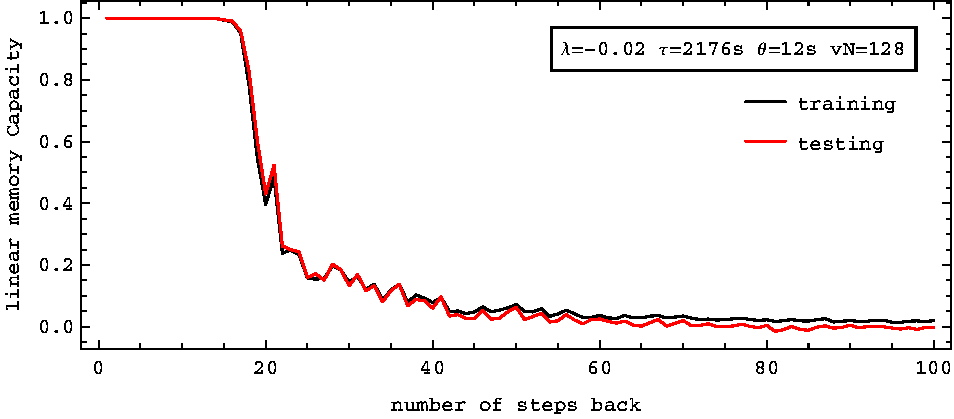
\includegraphics[width=0.99\linewidth]{pics/linearMemoryCurveN1}
	\caption{The linear memory capacities for varying steps into the past. The system is able to perfectly reproduce inputs up until $12$ steps into the past. $N=1, vN=128, \lambda=-0.02, \omega=1, \gamma=-0.1, \theta=12, \tau=2176$. }
	\label{fig:linearMemoryRecallCurveN1}
\end{figure}

\begin{figure}
	\centering
	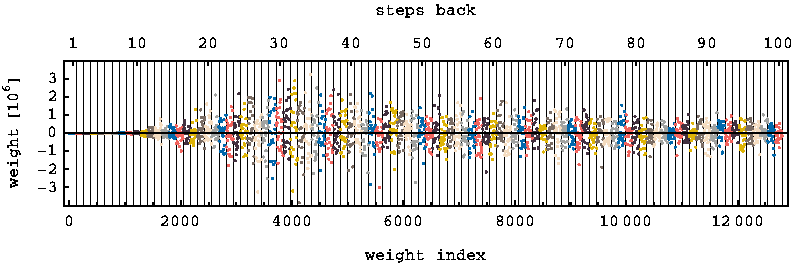
\includegraphics[width=0.99\linewidth]{pics/weight_plot}
	\caption{All weights $W_{i,s}$ attained through linear regression of the linear memory recalls $s \in [1,100]$ steps back. The system was a unidirectional ring with of $N_{real}=8$ and $N_{virtual}=16$ nodes. The total read-out dimension is $128$. For reconstruction of more recent inputs the inputs are small, but become enormous for inputs further in the past. This is the equivalent of "grasping at straws" as the system tries to extract information by multiplying microscopic fluctuations in the system state to linearily combine them to values between $[-1,1]$.}
	\label{fig:linearMemoryRecallWeights}
\end{figure}



\subsection{Legendre polynomials as Nonlinear Transformations}

In order to investigate the nonlinear transformation capabilities one can use Legendre polynomials  (Fig. \ref{fig:legendreDegrees}) in order to transform inputs $\textbf{U}(t)$.	Legendre Polynomials have the useful property of being orthonormal to every other Legendre polynomial within an interval $\left[-1,1\right]$. This makes them highly useful for measuring linearily independent nonlinear (but also linear) transformation capacities. Legendre polynomials $L_{d}(x)$ for degrees $d \in \{1-5\}$ are shown in fig.\ref{fig:legendreDegrees}. Depending on the definition they are scaled so that $L_{d}(1)=1$. The Legendre polynomial $L_{1}(x)$ is of course simply the identity, which makes it possible to investigate the linear memory capacity also.

The idea of measuring nonlinear (as well as linear) transformation capacities through the means of Legendre polynomials is largely inspired from the publication \cite{DAM12}. Hence the terminology used in the latter shall be used here as well (where possible). 

We start by defining $u^{-h}(t) = (u(t-h + 1), \dots, u(t))$ as the sequence of $h$ previous inputs. 
We start with an input $\textbf{u}$ which more precise will be $u^{-h}$ 


	\begin{equation}
	f:U^{h}\rightarrow \mathbb{R}:u^{-h}\rightarrow f\left[ u^{-h}\right]
	\label{eq:legendre_f_U_equaiont}
	\end{equation}
A function $f$ transforms inputs 


All nonlinear transformations of an input sequence $\textbf{U}^{h}$ can be expressed as a linear combination of Legendre  polynomials with $h$ being the number of data points already fed into the system. With inputs in $\textbf{U}^{h}$ it is necessary to test all combinations. To elaborate: 
For a singular Legendre polynomial $L_{d_{1}}(\textbf{U}(t_1))$ with degree $d_1$ all values of $t_1$ have to be tested.
For the product of $2$ Legendre polynomials $L_{d_{1}}(\textbf{U}(t_1))$ and $L_{d_{2}}(\textbf{U}(t_2))$ with degrees $d_1$ and $d_2$ all combinations of $\textbf{U}(t_1)$ and $\textbf{U}(t_2)$ have to be calculated.
For the product of $3$ Legendre polynomials $L_{d_{1}}(\textbf{U}(-t_1))$, $L_{d_{2}}(\textbf{U}(-t_2))$ and $L_{d_{3}}(\textbf{U}(-t_3))$ all combinations of ${t_1,t_2,t_3}$ have to be tested.

So for the Product of $n$ Legendre polynomials there exist permutations ${\textbf{d}}={d_1,d_2,...d_n}$ of.

\subsubsection{How to sum the right capacities}
In order to investigate the different nonlinear transformation capabilities of a system it is necessary to iterate over all possible combinations of Products of Legendre polynomials - an exercise in futility as the number of combinations is infinite. A number of restrictions need be applied to reduce number of calculations. A few (reasonable) assumptions are made:
\begin{itemize}
	\item capacities converge against zero for long recall distances -see Fig\ref{fig:linearMemoryRecallCurveN1}
	\item capacities for higher degrees converge against zero.
\end{itemize}
	But as we are not working in the limit of $K_{training} \rightarrow \infty$ the calculated capacities are subjected to noise. --see fig something. Summing over large amounts of noise results in too high capacities that can largely exceed the number of the theoretically limit which is the readout dimension. We avoid this by choosing the lowest possible threshold above noise level in order disregard all capacities beneath. For different lengths the distributions can be seen in Fig.\ref{fig:capacities_noise_distributions}.
	Accumulating capacities for different degrees $CM^1,CM^2,CM^3, ...$ is complicated through the existence of noisy capacity values.







\begin{figure}
	\centering
	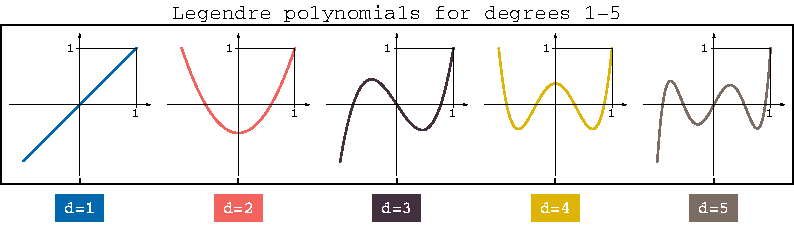
\includegraphics[width=0.99\linewidth]{pics/legendre_degrees}
	\caption{Legendre polynomials $L_{d}(u)$ for degrees $d \in \{1-5\}$ each shown for $u \in [-1,1]$ .}
	\label{fig:legendreDegrees}
\end{figure}

\begin{figure}\label{fig:legendre_transformation_predictions}
	\centering
	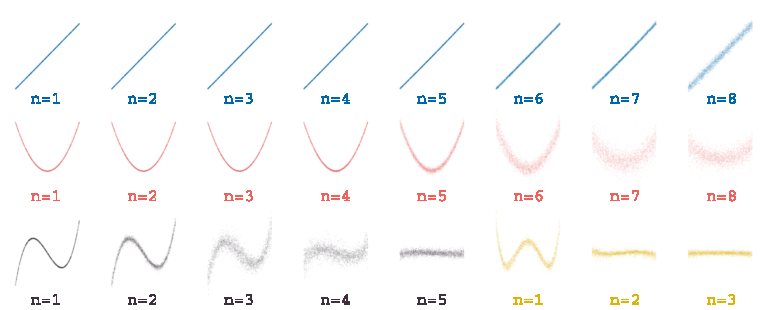
\includegraphics[width=15cm]{pics/predictions_pure_legendre}
	\caption{Using only the read-out state of the reservoir $\mathbf{x}(t)$ with some task-specific weight vectors $\mathbf{w}_{task}$ it is to an extent possible to predict the values $L_d(u(t-n T))$ with $n$ being the number of steps into the past. Here for different tasks and with different numbers of steps into the past $2500$ predictions based off $\mathbf{x}(t-nT)$ are plottet over values $u(t-n T)$. Reconstructing transformations on inputs further steps $n$ into the past results in poorer reconstructions. For higher degrees $d$ the results' qualities are also decaying faster - for $L_4$ (yellow	) the reconstructions only really works for $n=1$. The colors  of the different tasks are in accordance to Fig \ref{fig:legendreDegrees}.}
\end{figure}




They are used in Neural networks as well blabla citecite findfind. 
%\cite{VOELKER Legendre Memory Units: Continuous-TimeRepresentation in Recurrent Neural Networks}
%\begin{equation}


%\label{eq:legendrePolynomials}
%\end{equation}

\begin{figure}
	\centering
	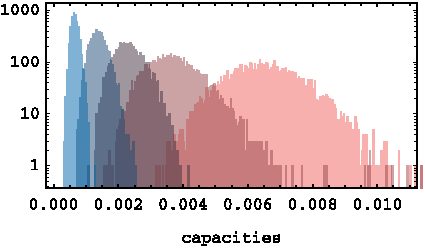
\includegraphics[width=8cm]{pics/noise_distributions}
	\caption{Varying distributions of the last $5000$ capacities (noise) are shown. From right to left the distributions resulted from $K_{training}=\{ 10^4, 2\cdot10^4, 3\cdot10^4, 5\cdot10^4, 10^5 \}$.}
	\label{fig:capacities_noise_distributions}
\end{figure}



\subsubsection{NARMA10 - the Nonlinear Autoregressive Moving Average Task}
\begin{equation}
A_{n+1} = 0.3 A_{n} + 0.05 A_{k}\left( \sum_{i=0}^{9} A_{k-9} \right) +1.5 u_{k-9} u_{k} + 0.1
\label{NARMA10equation}
\end{equation}

Lastly, the performance was investigated by measuring its capacity to compute the NARMA10 task. The Nonlinear Autoregressive Moving Average Task \cite{HER12} is used in many publications as a benchmark. The sequence is calculated using an average of its last $10$ steps while also being fed a product of a sequence $u(t)$ taken at two different positions. In order to calculate the NARMA10 sequence one needs memory $10$ steps (hence the "10") into the past as well as nonlinear transformation capacities. Recently it has been shown that the task is not ideal as its difficulty depends non-trivially on the shape of the distribution used \cite{KUB19}. In certain situations $A$ will quickly grow to $\infty$ when fed a sequence $u$ with a particularly large recent average. In order to avoid this $A_{n+1}$ has to be capped at $1$ which might be seen as a band aid rather than an elegant solution.
The NARMA10 sequence is created by the iterative formula given by \ref{NARMA10equation}. It is fed $2$ inputs from a sequence $u$ which is drawn from a uniform distribution $U \in [0,0.5]$.



\begin{figure}[h]
	\centering
	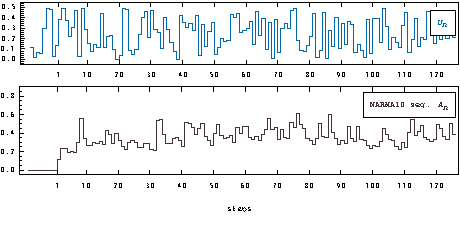
\includegraphics[width=13cm]{pics/narma_vis}
	\caption{Example for a uniformly drawn random sequence $U_n \in [0,0.5]$ that is used to create a Narma10 sequence $A_n$ with it. Here $A=0$ for $n<1$.}
	\label{fig:narma_vis}
\end{figure}
%here schöne plots mit narma.
	
	
	
	%order:
	%reservoir condition - fading memory etc.

\subsection{Stuart-Landau-Oscillator}
	\subsubsection{uncoupled version}
	The Stuart-Landau oscillator is a dynamical system often used to model basic class 1 lasers i.e. laser systems that do not exhibit pulsing or chaotic behavior (some refs). It can be written either as a single complex differential equation (\ref{eq:stuartlandauequation}) or a set of two equations written in polar coordinates (\ref{eq:stuartlandauequation_polar}). From the equation in polar coordinates easy to see that the equation has rotational symmetry as the radial differential equation does not change with the dynamical variable $\phi$. The Parameter $\lambda$ is often called the \emph{pump current} in accordance to its practical meaning.

\begin{equation}	
	\dot{z} = (\lambda +  i \omega + \gamma |z|^2 ) \; z
	\label{eq:stuartlandauequation}		
\end{equation}

\begin{equation}
	\begin{split}
	\dot{r} & = \lambda r + \operatorname{Re} (\gamma) \; r^{3} \\
	\dot{\phi} &= \omega + \operatorname{Im}(\gamma) \; r^{2} 
	\end{split}
	\label{eq:stuartlandauequation_polar}
\end{equation}

	For the radial dynamical variable the Stuart-Landau oscillator has two fixed points where the derivative $\dot{r}$ vanishes $r = 0$ and $r = \sqrt{-\lambda /\operatorname{Re}(\gamma)}$ whose stability depends on $\lambda$ and $\operatorname{Re}(\gamma)$. For $\operatorname{Re}(\gamma) < 0 $ (supercritical case).


\begin{figure}
	\centering
	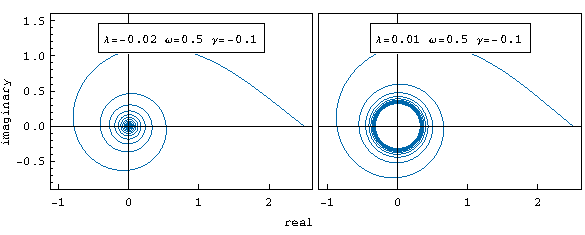
\includegraphics[width=0.99\linewidth]{pics/stuart_landau_complex_Focus_LC}
	\caption{$2$ very basic scenarios of the Stuart-Landau oscillator: Decay towards a single fixed point (off-state, left) or towards a stable oscillating state (limit cycle, right).}
	\label{fig:stuart_spiral}
	%nicht mehr
	%stuart_landau_basic.nb
\end{figure}


\subsubsection{Stuart-Landau with delay coupling}

	Introducing a coupling delay --- a "feedback loop" --- drastically increases complexity of the dynamic system. The phase-space dimension for a single delay-coupled Stuart-Landau oscillator (Fig.:\ref{eq:stuartlandauequation_delayed_driven} with $G=0$) becomes infinite. The reason for this instantaneous growth of complexity is that the initial condition $z_o = z(t_0)$ now becomes a function defined over the the interval $[t_0 - \tau,t_0]$. As the number of possible functions defined over $[t_0-\tau,t_0]$ is $\infty$, so becomes the dimension of phase space.  
	
	Finding periodic solutions and investigating their stability becomes complex and is its own field of research. One particular complication that results from introducing delay is that of growing multistability through increasing the delay time $\tau$.
	In \cite{YAN09, CHO09} multistability in delay systems are investigated, specifically for Stuart-Landau oscillators. The method is adapted to fit in this work and to account the value $\gamma < 0$ and for coupling strength $\kappa$ and coupling phase $\phi$. Let us consider the rotating wave solution $z(t) = r e^{i \Omega t}$ for \ref{eq:stuartlandauequation_delayed_driven} (with $G=0$, $Im(\gamma)=0$):

	\begin{equation}
	z(t) = r e^{i \Omega t}
	\end{equation}

	substituting $z$ in \ref{eq:stuartlandauequation_delayed_driven}  we gain:
	
	\begin{equation}
		i \Omega = (\lambda + i\omega + \gamma r^2) + \kappa e^{\phi-i \Omega \tau} 
	\end{equation}

	\subsubsection{Variing pump current}

\begin{figure}
	\centering
	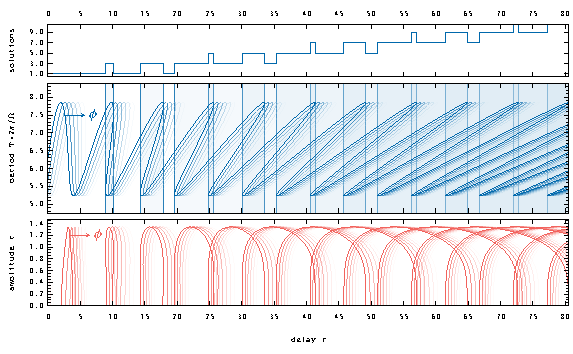
\includegraphics[width=15cm]{pics/stuart_landau_delaycoupled_per_amp}
	\caption{The solutions of (\ref{eq:stuartlandauequation_delayed_driven}) with $\lambda=0.02$, $\omega=1$, $\gamma=-0.1$,$\kappa=0.2$, $\phi=0$ (solutions for $\phi> 0$ are hinted). (top) Larger $\tau$ result in greater number of solutions. (middle:) relationship of $\tau$ and period $T$ of a rotating wave solutions. Areas of multiple solutions are colored lightly blue. For greater $\tau$ these areas increasingly overlap resulting in higher multistability. (bottom) parts where solutions $r \in \mathbb{R^+}$ exist (physical solutions with $r>0$). For higher $\tau$ multiple amplitude levels are possible depending on the system's state.}
	\label{fig:periodic_solutions_delay_coupled}
\end{figure}



The limit cycle (LC) which is shown in fig \ref{fig:stuart_spiral} is depending on the ratio or $\lambda$ and $Re \left[\gamma \right]$.


As can be seen in (eq. \ref{eq:stuartlandauequation}), the equation has a linear and a nonlinear term regarding the absolute value of $z$.


\begin{equation}	
\dot{z} = (\lambda + G J(t) + i \omega + \gamma |z|^2 ) \; z + \kappa e^{i \phi} z(t-\tau)
\label{eq:stuartlandauequation_delayed_driven}		
\end{equation}

In this work we use a Stuart-Landau oscillator that has a varying bifurcation parameter $\hat{\lambda}(t)$ and a delayed feedback term $\kappa e^{i\phi}z(t-\tau)$. In our case $\hat{\lambda}(t)$ will always be an offset with only slight variations. We will therefore simply write  $\hat{\lambda}(t) = \lambda + G J(t)$ with $G \in \mathbb{R}$ being in the order of or exactly equal to $0.01$ (if not stated otherwise). The input signal $J(t)$ will be the actual variation that is used to feed data into the system (see Fig. \ref{fig:signal_mask_vis}). 

\begin{figure}
	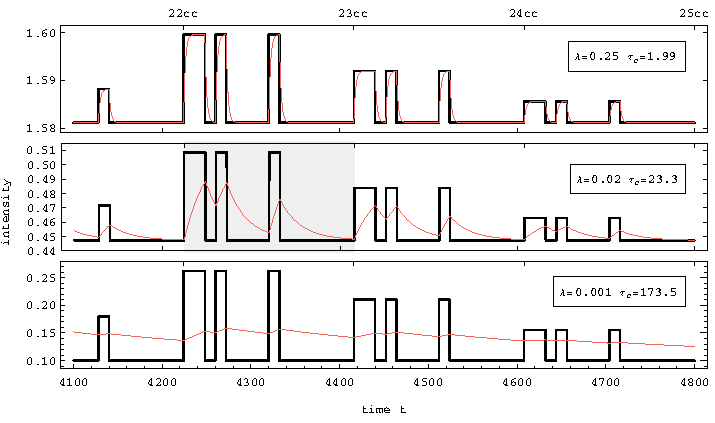
\includegraphics[width=15cm]{pics/different_lambda_values}
	\caption{Different values for $\lambda$ influence how fast the system's intensity \textcolor{myred}{\rule[2pt]{25pt}{2.5pt}} is responding to a given input signal. For a large value of $\lambda=0.25$ (top) the system's intensity almost instantaneously decays towards the expected limit cycle LC \rule[2pt]{25pt}{2.5pt}. The system is therefore determined exclusively by the current pump current. For intermediate values e.g. $\lambda=0.02$ (mid) the system's response is slower and can keep information longer. Very small values e.g. $\lambda=0.001$ (bottom) make the system respond too slow to react to a given input signal. For each solution the characteristic timescales $\tau_{c}$ were gained by fitting a function $a e^{-t/\tau_{c}} + b$ to $|z(t)|^2$ with $t \in [4332,4400]$.}
	\label{fig:stuart_driven_landau_lambda_impact}
\end{figure}

\begin{figure}
	\centering
	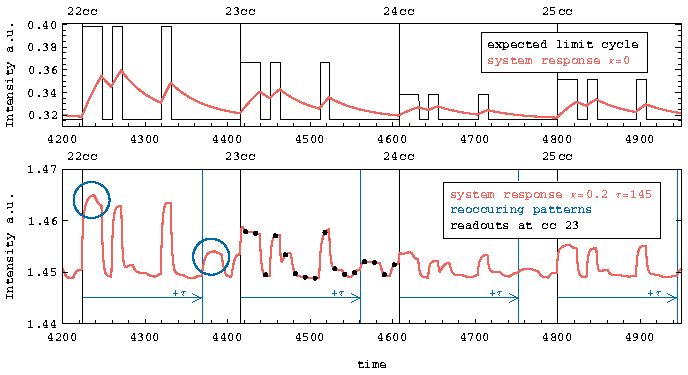
\includegraphics[width=15cm]{pics/driven_and_delayed}
	\caption{$|z|^{2}(t)$ of a driven Stuart-Landau oscillator with delayed feedback. Each clockcycle the system state is read out once per virtual node (red dots on the left). With delayed feedback patterns reappear after delay time $\tau$: the bump within the right blue rectangle is not caused by the input signal (above), but is an echo of the bump within the left blue rectangle. Without the delayed feedback ($\kappa=0$) the system response can be seen in the grey area in Fig.\ref{fig:stuart_driven_landau_lambda_impact}}
	\label{fig:driven_and_delayed}
\end{figure}

In Fig. \ref{fig:driven_and_delayed} a solution for $|z(t)|$ with and without delayed feedback is shown. Without it the intensity is exponentially decaying towards the new limit cycle (in black). With delayed feedback (bottom) previous inputs reappear: The little bump encased in the second blue box is information that is fed back into the system. Usually the information isn't as visible or locally distinct, but a linear combination of all given readouts.

\begin{figure}\label{fig:input_capacities}\centering
	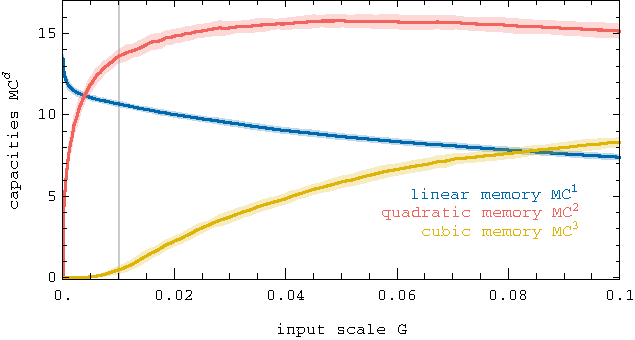
\includegraphics[width=12cm]{pics/input_capacities}
	\caption{Capacity means and standard deviations from $20$ random realizations per input scale $G$ respectively (variing masks/initial state). $G$ strongly determines the reservoir performance of different tasks. Parameters: $N_r=1, \lambda=-0.02, \omega=1, \gamma=-0.1, \tau=68, N_v=64, \theta=3/4, T=N_v \theta = 48$. In this work an input scaling of $G=0.01$ (indicated as vertical line) was used at all times.}
\end{figure}


\subsection{Networks}

	\begin{figure}
		\centering
		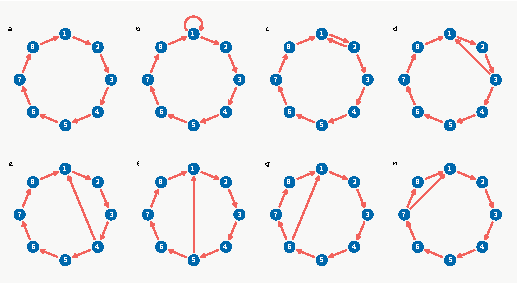
\includegraphics[width=12cm]{pics/graph_plot}
		\caption{example graph}
		\label{fig:example_graph}
	\end{figure}

Vertices blabla \
Edges blabla. \

	\subsubsection{circulant Matrix}
    A circulant matrix has the same entries its row vectors, but with its entries rotated one element to the right relative to the previous row.

    
\subsection{virtual Nodes and multiplexing}
	idea of multiplexing originally introduced by Appeltant et al. in \cite{APP11}. 
	originally with binary mask (on/off), variations are uniform masks or noise masks.
	here: papers for explanation!
	\cite{KUR18}?
	\cite{APP14} comparison of masks (binary<uniform<noise(with high cutoff))
	\cite{STE20} // off-resonance = better! --> reason for choosing 17 * 12.
	
	By multiplexing the input signal one can create virtual nodes in a network. The analogy to a real network can be best understood if the input signal is masked with a binary mask containing only values of either $0$ or $1$.
	
	Different Mask types: discrete values with constant interpolation: binary, uniform - easy to implement)
	continuous: any function or repeating noise-patterns. (more difficult, but )

	here add dependency of total linear memory on number of nodes and virtal nodes.
	
	\begin{figure}
		\centering
		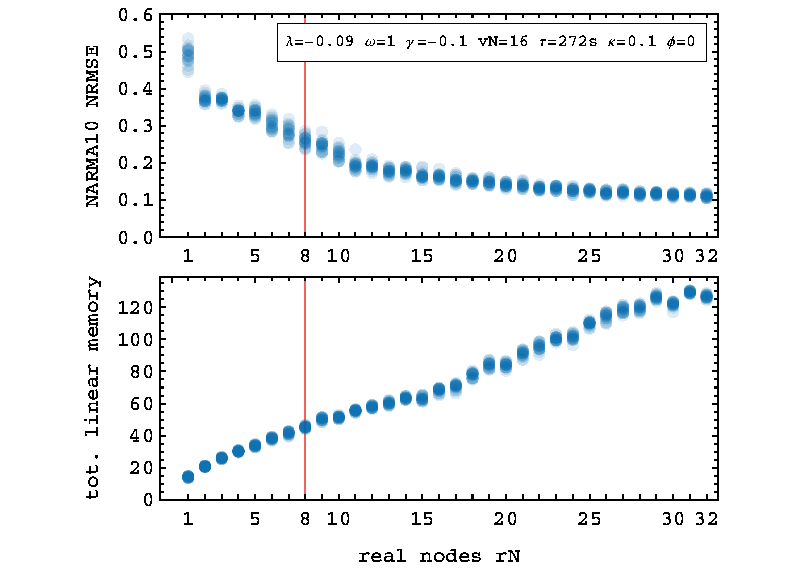
\includegraphics[width=0.9\linewidth]{pics/rNplot}
		\caption{changing rc performance for increasing number or real nodes $rN$ in unidirectianally coupled ring networks. (see some plot).}
		\label{fig:rN_1-32}
	\end{figure}

	\begin{figure}
		\centering
		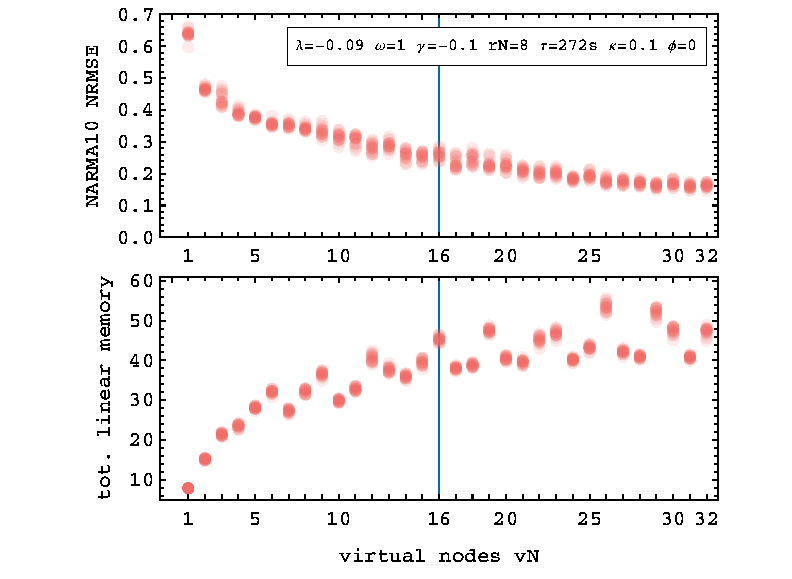
\includegraphics[width=15cm]{pics/vNplot}
		\caption{changing rc performance for increasing number or virtual nodes $rN$ in unidirectionally coupled ring networks. (see some plot).}
		\label{fig:vN_1-32}
	\end{figure}


\begin{figure}
	\centering
	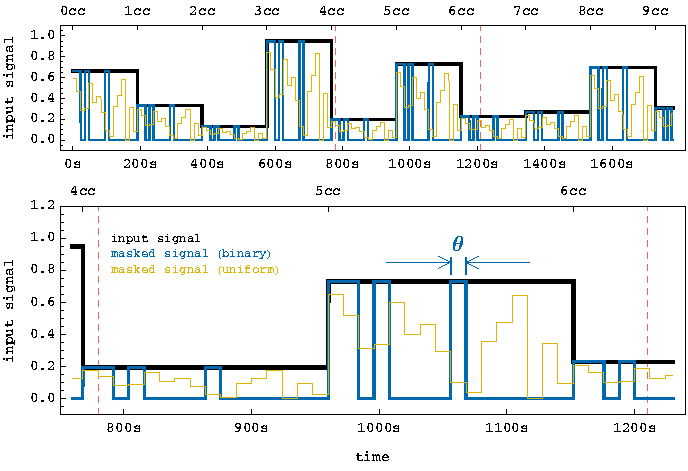
\includegraphics[width=15cm]{pics/signal_mask_vis}
	\caption{A timeseries of data points \textcolor{myred}{\color{myred}$\sbullet[2]$}\,with its constant-interpolated signal between samples \rule[2pt]{25pt}{2.5pt}\, and the corresponding masked signals \textcolor{myblue}{\rule[2pt]{25pt}{2.5pt}} and \textcolor{myyellow}{\rule[2pt]{25pt}{2.5pt}}\,. The mask times (or lengths) are usually defined as input period $T$ or clockcycle (indicated $T$, upper major ticks) and the time per virtual node called $\theta$ (upper minor ticks). Here $\theta = 12$ and $T = 16 \theta = 272 $}
	\label{fig:signal_mask_vis}
	%feedInVis_stuartlandau.nb
\end{figure}



\subsection{Dynamics of rings of stuart landau oscillators}
	pony-states (von André)
	


\subsection{Implementation details}

In order to save time some adjustments were made where possible. The NARMA10 task uses inputs $u_{n}$ drawn from a uniform distribution $U \in [0,0.5]$ to calculate sequence members $A_{n}$. The (non-)linear memory capacities gained through the Legendre polynomials rely on inputs $u$ drawn from a symmetric unform distribution $U \in [-1,1]$. To avoid processing two sets of calculations - one with NARMA10 and one with the Legendre task both tasks were made using the same sequence $u \in [-1,1]$. For NARMA10 the sequence $u$ was mapped with the function $m$ (\ref{eq:mapping_u}) onto $m(u)$. 

\begin{equation}
	m: [-1,1] \rightarrow [0,0.5] : u \rightarrow (u + 1)/4
	\label{eq:mapping_u}
\end{equation}



\subsection{mathematical details}

Calculating memory capacities can be either done through solving a the system of linear equations or by calculating the covariances of targets and predictions. 

\subsubsection{integration}
Integration was through the Runge Kutta method of fourth degree with a fixed stepsize. Since we are dealing with delay differential equations, we run into a problem when as the delayed state $z(t-\tau)$ is only available as discrete values. In order to calculate $k_2$ and $k_3$ an interpolated value for $z(t-\tau+h/2)$ has to be approximated from the existing values $z(t-\tau)$ and $z(t-\tau+h)$. Linear interpolation should be avoided as the error resulting from the poor interpolation method would be of higher order than the error of the fourth order Runge Kutta method. In general  
\cite{FIL89}

\cite{NEV76} // mabye not

Solving a system of linear equations.
Design matrix or State matrix $S$.

\begin{figure}
	\begin{equation}
	S=\begin{pmatrix}
	x_{1}^{1} & \dots & x_{1}^{D} & 1 \\
	\vdots & & \vdots & \vdots \\
	x_{K}^{1} & \dots & x_{K}^{D} & 1 \\
	\end{pmatrix}
=
	\begin{pmatrix}
	x_{1}^{1} & \dots & x_{1}^{K} & 1 \\
	\vdots & & \vdots & \vdots \\
	x_{1}^{1} & \dots & x_{1}^{K} & 1 \\
	\end{pmatrix}
	\end{equation}
\end{figure}

Meaning of values inside the design matrix $S$.


\begin{figure}
	\centering
	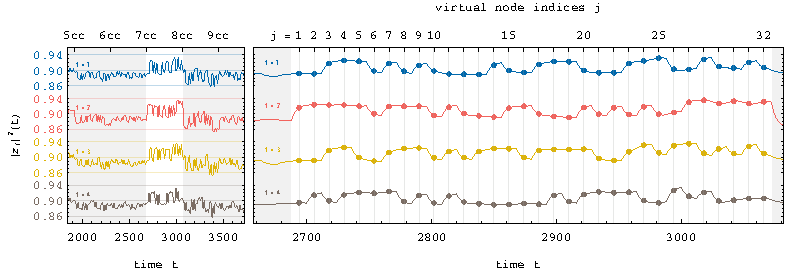
\includegraphics[width=15cm]{pics/driven_ts_statematrix}
	\caption{The traces $|z_{i}|(t)$ with $i=1,2,3,4$ ($\textcolor{myblue}{\sbullet[1.5]}\textcolor{myred}{\sbullet[1.5]}\textcolor{myyellow}{\sbullet[1.5]}\textcolor{mybrown}{\sbullet[1.5]}$) of a system with $N_{r}=4$ nodes and virtualization factor $N_{v}=32$. The readouts $\textbf{x}(7T)$ for input period $T=[7cc,8cc]$ are indicated by the dots on the right. All dots together make one row in the state matrix $\textbf{S}$.}
	\label{fig:ts_vn_for_statematrix}
\end{figure}


\begin{equation}
x_{ij}^{k} = |z_{i}(k T + j\theta)|\\
\end{equation}

\begin{align}
\mathbf{S}=&
\setlength{\arraycolsep}{0.0pt}
\left(\begin{array}{cccccccc c cccc}
\textcolor{myblue}{\sbullet[1.5]^{1}_1}&\textcolor{myred}{\sbullet[1.5]^{1}_1}&\textcolor{myyellow}{\sbullet[1.5]^{1}_1}&\textcolor{mybrown}{\sbullet[1.5]^{1}_1}&\textcolor{myblue}{\sbullet[1.5]^{1}_2}&\textcolor{myred}{\sbullet[1.5]^{1}_2}&\textcolor{myyellow}{\sbullet[1.5]^{1}_2}&\textcolor{mybrown}{\sbullet[1.5]^{1}_2}&\dots&\textcolor{myblue}{\sbullet[1.5]^{1}_{N_v}}&\textcolor{myred}{\sbullet[1.5]^{1}_{N_v}}&\textcolor{myyellow}{\sbullet[1.5]^{1}_{N_v}}&\textcolor{mybrown}{\sbullet[1.5]^{1}_{N_v}}\\
\textcolor{myblue}{\sbullet[1.5]^{2}_1}&\textcolor{myred}{\sbullet[1.5]^{2}_1}&\textcolor{myyellow}{\sbullet[1.5]^{2}_1}&\textcolor{mybrown}{\sbullet[1.5]^{2}_1}&\textcolor{myblue}{\sbullet[1.5]^{2}_2}&\textcolor{myred}{\sbullet[1.5]^{2}_2}&\textcolor{myyellow}{\sbullet[1.5]^{2}_2}&\textcolor{mybrown}{\sbullet[1.5]^{2}_2}&\dots&\textcolor{myblue}{\sbullet[1.5]^{2}_{N_v}}&\textcolor{myred}{\sbullet[1.5]^{2}_{N_v}}&\textcolor{myyellow}{\sbullet[1.5]^{2}_{N_v}}&\textcolor{mybrown}{\sbullet[1.5]^{2}_{N_v}}\\
\textcolor{myblue}{\vdots}&\textcolor{myred}{\vdots}&\textcolor{myyellow}{\vdots}&\textcolor{mybrown}{\vdots}&\textcolor{myblue}{\vdots}&\textcolor{myred}{\vdots}&\textcolor{myyellow}{\vdots}&\textcolor{mybrown}{\vdots}& &\textcolor{myblue}{\vdots}&\textcolor{myred}{\vdots}&\textcolor{myyellow}{\vdots}&\textcolor{mybrown}{\vdots}\\
\textcolor{myblue}{\sbullet[1.5]^{k}_1}&\textcolor{myred}{\sbullet[1.5]^{k}_1}&\textcolor{myyellow}{\sbullet[1.5]^{k}_1}&\textcolor{mybrown}{\sbullet[1.5]^{k}_1}&\textcolor{myblue}{\sbullet[1.5]^{k}_2}&\textcolor{myred}{\sbullet[1.5]^{k}_2}&\textcolor{myyellow}{\sbullet[1.5]^{k}_2}&\textcolor{mybrown}{\sbullet[1.5]^{k}_2}&\dots&\textcolor{myblue}{\sbullet[1.5]^{k}_{N_v}}&\textcolor{myred}{\sbullet[1.5]^{k}_{N_v}}&\textcolor{myyellow}{\sbullet[1.5]^{k}_{N_v}}&\textcolor{mybrown}{\sbullet[1.5]^{k}_{N_v}}\\
\textcolor{myblue}{\vdots}&\textcolor{myred}{\vdots}&\textcolor{myyellow}{\vdots}&\textcolor{mybrown}{\vdots}&\textcolor{myblue}{\vdots}&\textcolor{myred}{\vdots}&\textcolor{myyellow}{\vdots}&\textcolor{mybrown}{\vdots}& &\textcolor{myblue}{\vdots}&\textcolor{myred}{\vdots}&\textcolor{myyellow}{\vdots}&\textcolor{mybrown}{\vdots}\\
\textcolor{myblue}{\sbullet[1.5]^{K}_1}&\textcolor{myred}{\sbullet[1.5]^{K}_1}&\textcolor{myyellow}{\sbullet[1.5]^{K}_1}&\textcolor{mybrown}{\sbullet[1.5]^{K}_1}&\textcolor{myblue}{\sbullet[1.5]^{K}_2}&\textcolor{myred}{\sbullet[1.5]^{K}_2}&\textcolor{myyellow}{\sbullet[1.5]^{K}_2}&\textcolor{mybrown}{\sbullet[1.5]^{K}_2}&\dots&\textcolor{myblue}{\sbullet[1.5]^{K}_{N_v}}&\textcolor{myred}{\sbullet[1.5]^{K}_{N_v}}&\textcolor{myyellow}{\sbullet[1.5]^{K}_{N_v}}&\textcolor{mybrown}{\sbullet[1.5]^{K}_{N_v}}\\
\end{array}\right)  \\[0.75cm]
\mathbf{S}_{\mathbf{\neg}\textcolor{myred}{\sbullet[1]}}=&
\setlength{\arraycolsep}{0.0pt}
\left(\begin{array}{ccccccc ccc}
\textcolor{myblue}{\sbullet[1.5]^{1}_1}&\textcolor{myyellow}{\sbullet[1.5]^{1}_1}&\textcolor{mybrown}{\sbullet[1.5]^{1}_1}&\textcolor{myblue}{\sbullet[1.5]^{1}_2}&\textcolor{myyellow}{\sbullet[1.5]^{1}_2}&\textcolor{mybrown}{\sbullet[1.5]^{1}_2}&\dots&\textcolor{myblue}{\sbullet[1.5]^{1}_{N_v}}&\textcolor{myyellow}{\sbullet[1.5]^{1}_{N_v}}&\textcolor{mybrown}{\sbullet[1.5]^{1}_{N_v}}\\
\textcolor{myblue}{\sbullet[1.5]^{2}_1}&\textcolor{myyellow}{\sbullet[1.5]^{2}_1}&\textcolor{mybrown}{\sbullet[1.5]^{2}_1}&\textcolor{myblue}{\sbullet[1.5]^{2}_2}&\textcolor{myyellow}{\sbullet[1.5]^{2}_2}&\textcolor{mybrown}{\sbullet[1.5]^{2}_2}&\dots&\textcolor{myblue}{\sbullet[1.5]^{2}_{N_v}}&\textcolor{myyellow}{\sbullet[1.5]^{2}_{N_v}}&\textcolor{mybrown}{\sbullet[1.5]^{2}_{N_v}}\\
\textcolor{myblue}{\vdots}&\textcolor{myyellow}{\vdots}&\textcolor{mybrown}{\vdots}&\textcolor{myblue}{\vdots}&\textcolor{myyellow}{\vdots}&\textcolor{mybrown}{\vdots}& &\textcolor{myblue}{\vdots}&\textcolor{myyellow}{\vdots}&\textcolor{mybrown}{\vdots} \\
\textcolor{myblue}{\sbullet[1.5]^{k}_1}&\textcolor{myyellow}{\sbullet[1.5]^{k}_1}&\textcolor{mybrown}{\sbullet[1.5]^{k}_1}&\textcolor{myblue}{\sbullet[1.5]^{k}_2}&\textcolor{myyellow}{\sbullet[1.5]^{k}_2}&\textcolor{mybrown}{\sbullet[1.5]^{k}_2}&\dots&\textcolor{myblue}{\sbullet[1.5]^{k}_{N_v}}&\textcolor{myyellow}{\sbullet[1.5]^{k}_{N_v}}&\textcolor{mybrown}{\sbullet[1.5]^{k}_{N_v}}\\
\textcolor{myblue}{\vdots}&\textcolor{myyellow}{\vdots}&\textcolor{mybrown}{\vdots}&\textcolor{myblue}{\vdots}&\textcolor{myyellow}{\vdots}&\textcolor{mybrown}{\vdots}& &\textcolor{myblue}{\vdots}&\textcolor{myyellow}{\vdots}&\textcolor{mybrown}{\vdots} \\
\textcolor{myblue}{\sbullet[1.5]^{K}_1}&\textcolor{myyellow}{\sbullet[1.5]^{K}_1}&\textcolor{mybrown}{\sbullet[1.5]^{K}_1}&\textcolor{myblue}{\sbullet[1.5]^{K}_2}&\textcolor{myyellow}{\sbullet[1.5]^{K}_2}&\textcolor{mybrown}{\sbullet[1.5]^{K}_2}&\dots&\textcolor{myblue}{\sbullet[1.5]^{K}_{N_v}}&\textcolor{myyellow}{\sbullet[1.5]^{K}_{N_v}}&\textcolor{mybrown}{\sbullet[1.5]^{K}_{N_v}} \label{eq:statematrix_fill_and_omit}\\
\end{array}\right)
\end{align}


\begin{equation}
\mathbf{S}_{\textcolor{myred}{\sbullet[1]}}=
\setlength{\arraycolsep}{-0.0pt}
\left(\begin{array}{ccc c}
\textcolor{myred}{\sbullet[1.5]^{1}_1}&\textcolor{myred}{\sbullet[1.5]^{1}_2}&\dots&\textcolor{myred}{\sbullet[1.5]^{1}_{N_v}}\\
\textcolor{myred}{\sbullet[1.5]^{2}_1}&\textcolor{myred}{\sbullet[1.5]^{2}_2}&\dots&\textcolor{myred}{\sbullet[1.5]^{2}_{N_v}}\\
\textcolor{myred}{\vdots}&\textcolor{myred}{\vdots}& &\textcolor{myred}{\vdots}\\
\textcolor{myred}{\sbullet[1.5]^{k}_1}&\textcolor{myred}{\sbullet[1.5]^{k}_2}&\dots&\textcolor{myred}{\sbullet[1.5]^{k}_{N_v}}\\
\textcolor{myred}{\vdots}&\textcolor{myred}{\vdots}& &\textcolor{myred}{\vdots}\\
\textcolor{myred}{\sbullet[1.5]^{K}_1}&\textcolor{myred}{\sbullet[1.5]^{K}_2}&\dots&\textcolor{myred}{\sbullet[1.5]^{K}_{N_v}}\\
\end{array}\right)
\label{eq:statematrix_fill_and_single}
\end{equation}


\ref{eq:statematrix_fill_and_omit} maybe not as figure ... 
The readouts $x^k_{ij}$ are performed during the numerical integration of $\mathbf{z(t)}$ and saved in the statematrix $\mathbf{S}$. Here the nodes $i= 1,2,3,4 $ ($\textcolor{myblue}{\sbullet[1.5]}\textcolor{myred}{\sbullet[1.5]}\textcolor{myyellow}{\sbullet[1.5]}\textcolor{mybrown}{\sbullet[1.5]}$) are colored according to the example in Fig.\ref{fig:ts_vn_for_statematrix}. Row $k$ of $\mathbf{S}$ contains all readouts $x$ for the input period $k$ with $k \in [1,K]$. Each column corresponds to one virtual node of one real node. If we only select readouts from node $\textcolor{myred}{\sbullet[1.5]}$ we derive a new statematrix $\mathbf{S}_{\textcolor{myred}{\sbullet[1]}}$. By omitting readouts from $\textcolor{myred}{\sbullet[1.5]}$ (here $i=2$) we get  $\textbf{S}_{\neg \textcolor{myred}{\sbullet[1]}}$. 






	
	
% different stuart landau scenarios - hopf bifurcation